%%===========================================================%%
%%                                                           %%
%%                      Roman Pot Alignment                  %%
%%                                                           %%
%%===========================================================%%

\chapter{Apertures tuning in Geant4 simulation}\label{appendix:g4ApertureTuning}

\begin{figure}[hb]\centering%
\caption{The DX aperture envelopes fitted with circles before (left) and after (right) the DX offsets introduced in the Geant4 geometry.}\label{fig:aperturesWithFit}%
\parbox{0.495\textwidth}{
  \centering
  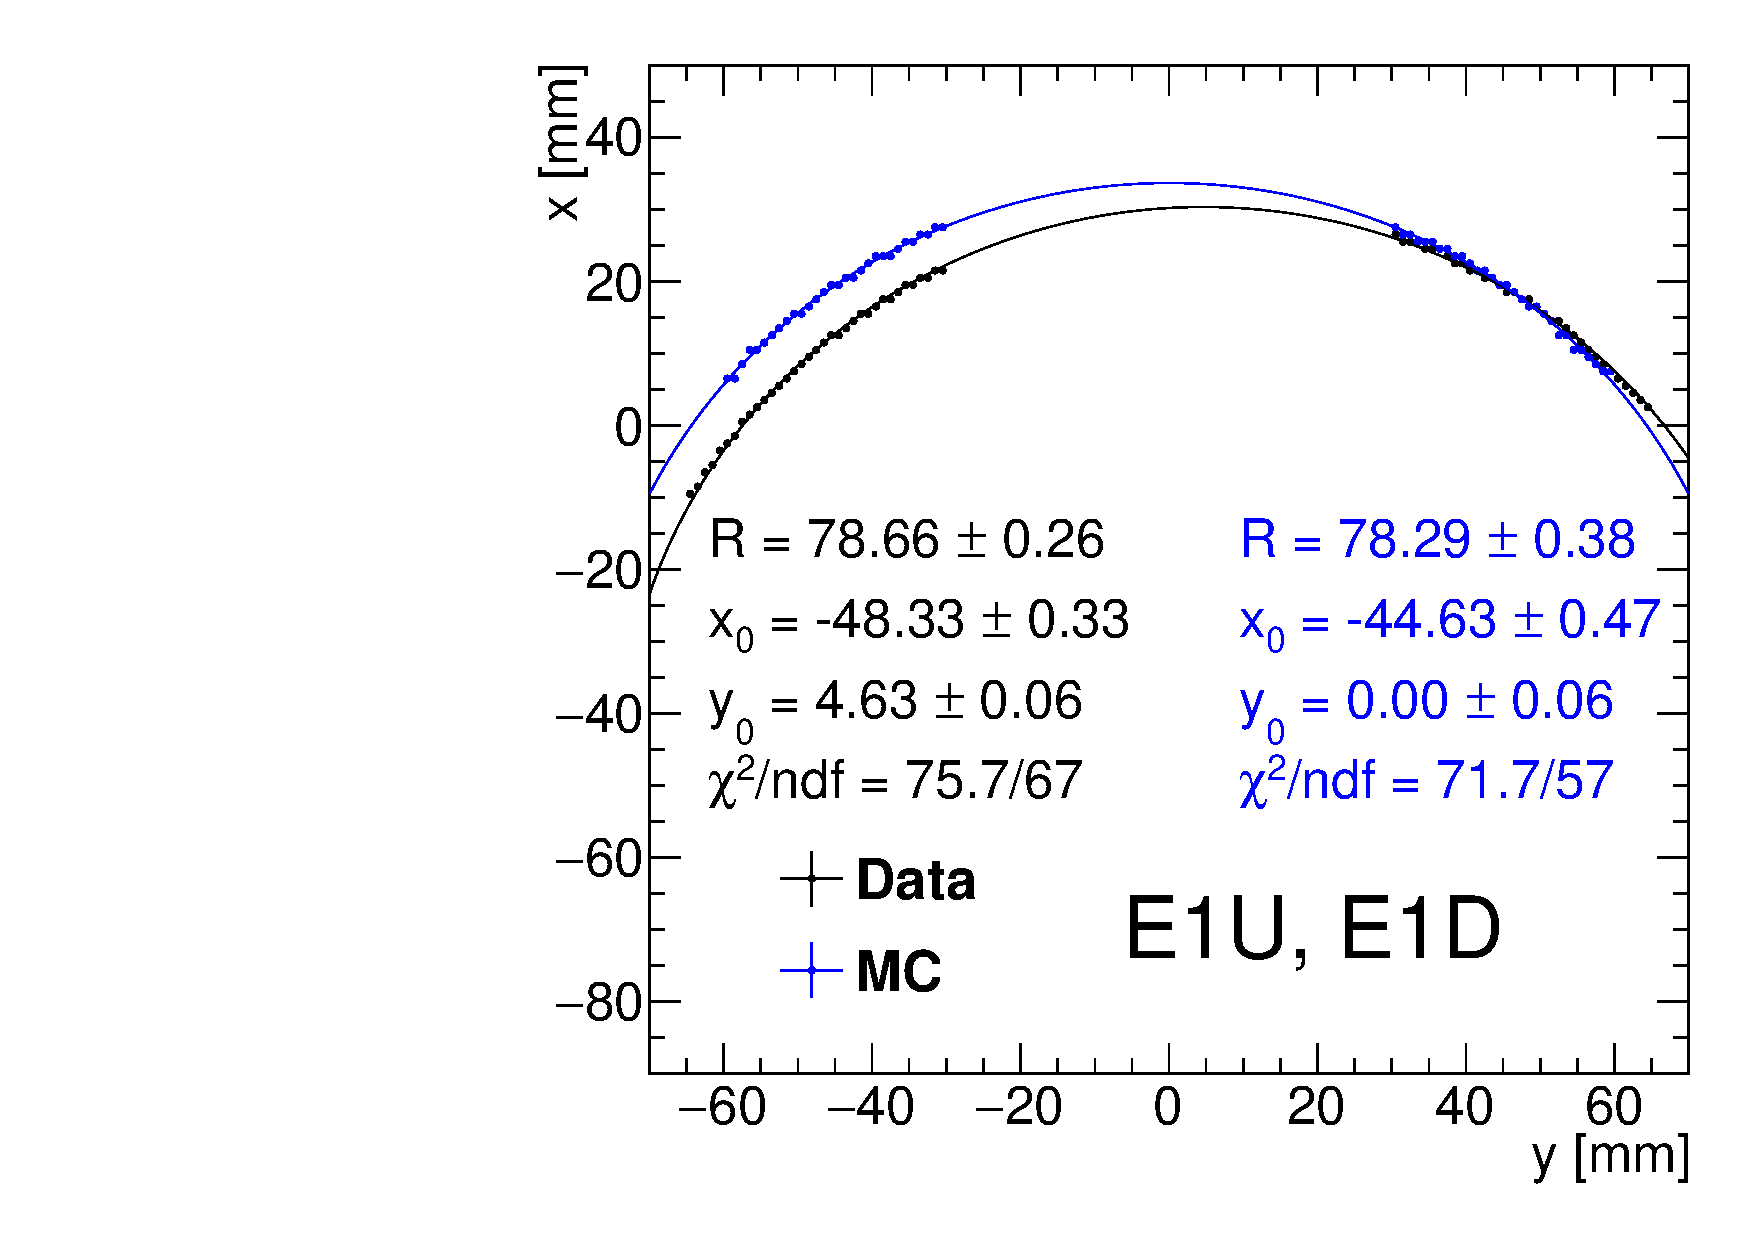
\includegraphics[width=\linewidth,page=1]{graphics/rpSim/Apertures_swapedAxes_withFit_beforeDxShift.pdf}\\[10pt]
  \includegraphics[width=\linewidth,page=2]{graphics/rpSim/Apertures_swapedAxes_withFit_beforeDxShift.pdf}
}~
\parbox{0.495\textwidth}{
  \centering
  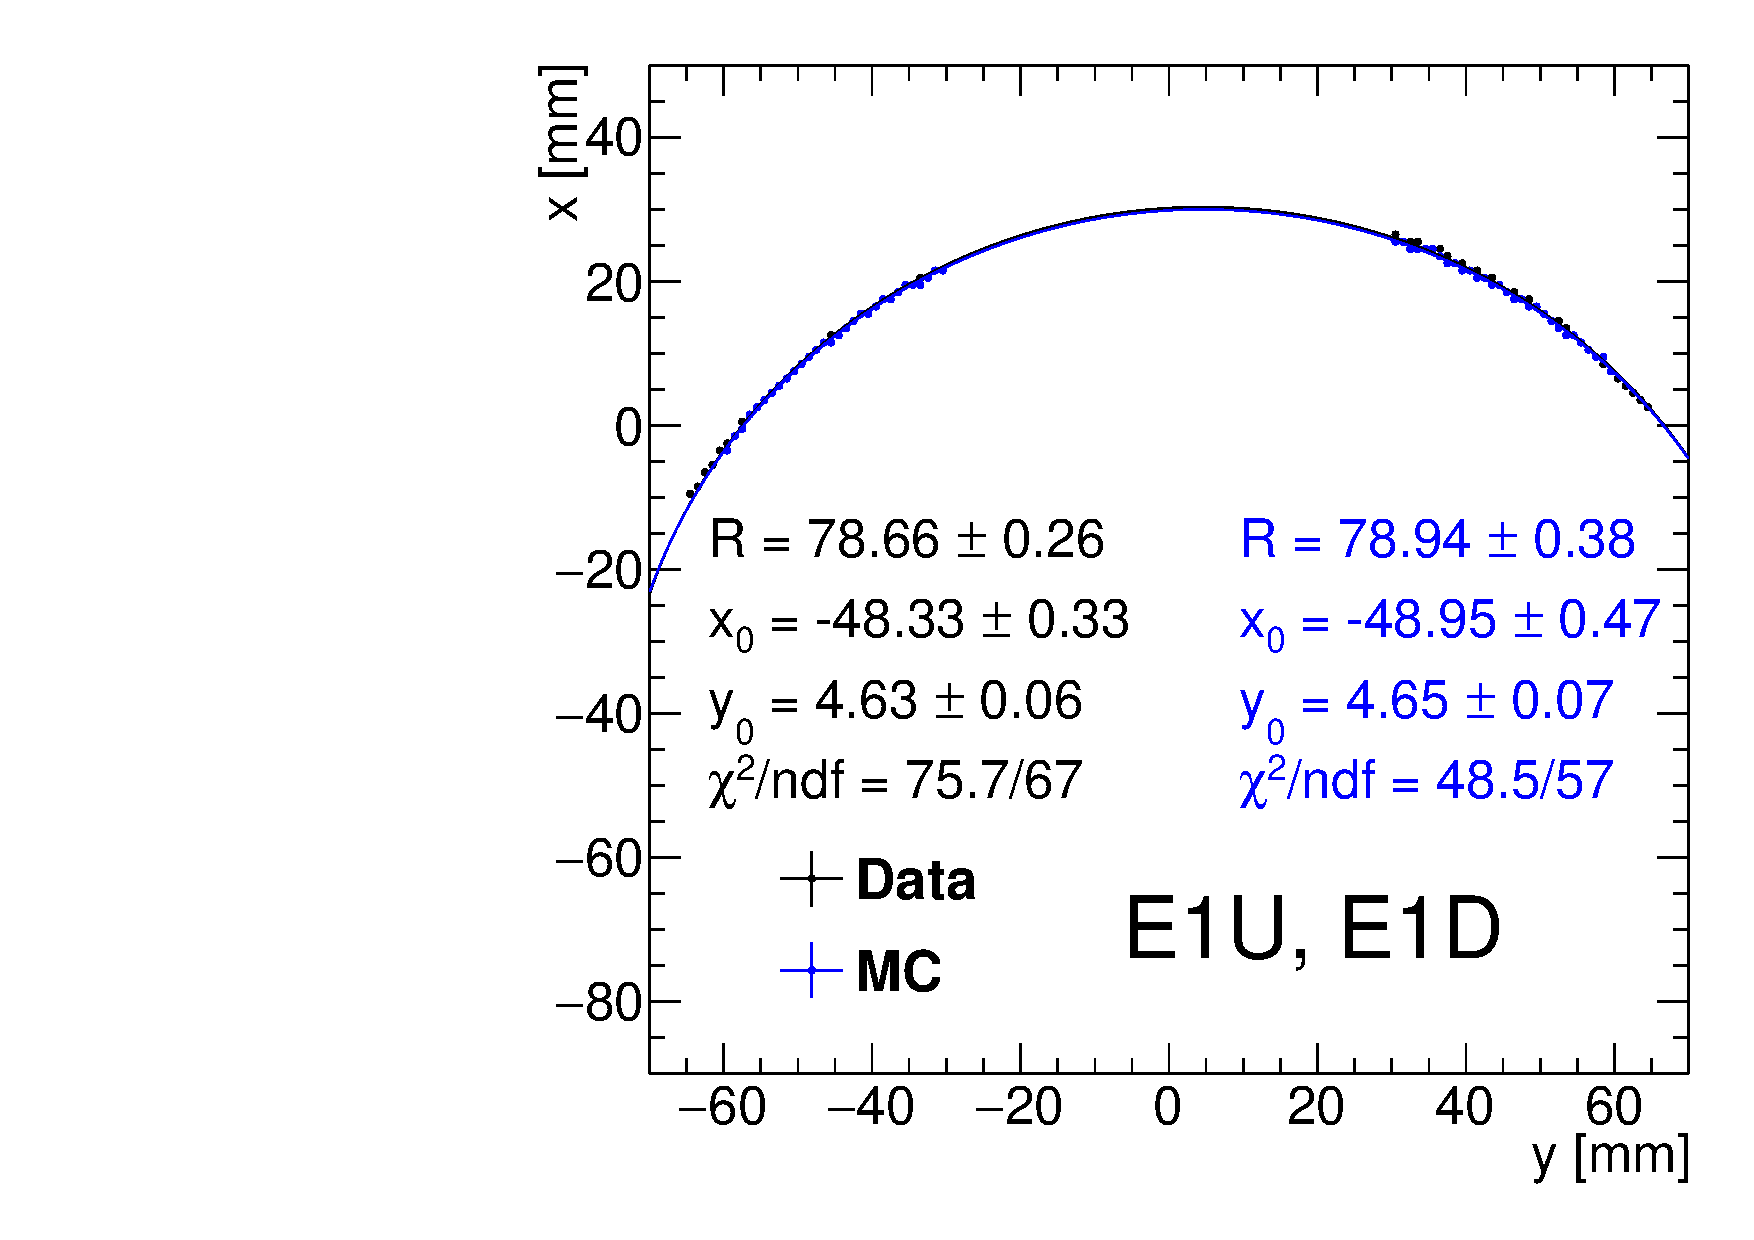
\includegraphics[width=\linewidth,page=1]{graphics/rpSim/Apertures_swapedAxes_withFit.pdf}\\[10pt]
  \includegraphics[width=\linewidth,page=2]{graphics/rpSim/Apertures_swapedAxes_withFit.pdf}
}%
\end{figure}

\begin{figure}[ht]\ContinuedFloat\centering%
	%\caption[Apertures.]{Apertures.}\label{fig:aperturesWithFit}%
	\parbox{0.495\textwidth}{
		\centering
		\includegraphics[width=\linewidth,page=3]{graphics/rpSim/Apertures_swapedAxes_withFit_beforeDxShift.pdf}\\[10pt]
		\includegraphics[width=\linewidth,page=4]{graphics/rpSim/Apertures_swapedAxes_withFit_beforeDxShift.pdf}
	}~
	\parbox{0.495\textwidth}{
		\centering
		\includegraphics[width=\linewidth,page=3]{graphics/rpSim/Apertures_swapedAxes_withFit.pdf}\\[10pt]
		\includegraphics[width=\linewidth,page=4]{graphics/rpSim/Apertures_swapedAxes_withFit.pdf}
	}%
\end{figure}


